
\chapter{Estado del arte}

\label{aprmaqvir}
La tecnología de virtualización y la computación en la nube son dos áreas de investigación muy activas. La investigación que produce estos campos es demasiada para enumerar. Cada una tiene múltiples conferencias de investigación. Por ejemplo, la ACM Symposium on Cloud Computing (SOCC) \cite{socc15} es uno de los lugares más conocidos en investigación de la computación en la nube y tecnologías de virtualización.\\
\\
La importancia de estas dos areas en la industria radica en que las nubes han transformado la forma de hacer computación. En general una empresa que use los servicios de una nube no necesita preocuparse tanto acerca de la administración de la infraestructura, las copias de seguridad, el mantenimiento, la depreciación, fiabilidad, rendimiento y tal vez de la seguridad. Estas tareas son ahora realizadas por los proveedores de la nube en otro lugar fuera de la empresa que los contrata.\\
\\
En la actualidad existen una gran oferta de nubes. Algunas de estas son públicas y están disponibles para cualquiera que esté dispuesto a pagar por el uso de los recursos, las demás son privadas para una organización. Del mismo modo, diferentes nubes ofrecen cosas diferentes. Algunas dan a sus usuarios el acceso a hardware físico, pero la mayoría permiten virtualizar sus entornos. Algunas ofrecen  las máquinas virtuales, desnudas o no, y nada más, pero otras ofrecen software que está listo para
utilizar y se pueden combinar de manera interesante, o plataformas que hacen que sea fácil para
sus usuarios desarrollar nuevos servicios \cite{tanembaum14}.\\
\\
En ese contexto, una de las principales características de la computación en la nube es la virtualización, la cual crea la ilusión de múltiples máquinas (virtuales), cada una potencialmente ejecuta un sistema operativo completamente, diferente usando el mismo hardware físico. La virtualización se puede aplicar a computadoras, sistemas operativos, dispositivos de almacenamiento de información, aplicaciones o redes. Esto permite que las empresas ejecuten mas de un sistema virtual, ademas de múltiples sistemas operativos y aplicaciones, en un único servidor, de esta manera se logra economía de escala y una mayor eficiencia.\\
\\
\section{Técnicas de Virtualización}
Actualmente predominan dos técnicas de virtualización. La primera técnica se denomina virtualización de hardware y consiste en que el software subyacente que ejecuta las máquinas virtuales conocido como hipervisor, crea y corre maquinas virtuales proporcionando una interfaz que es idéntica a la del servidor físico (también conocido como maquina anfitriona). El hipervisor, interactúa directamente con la CPU en el servidor físico, ofreciendo a cada uno de los servidores virtuales una total autonomía e independencia (Figura \ref{fig:hipervisor}). Incluso pueden coexistir en una misma maquina distintos servidores virtuales funcionando con distintos sistemas operativos. Esta técnica es la mas desarrollada y hay diferentes productos que cada fabricante ha ido desarrollando y adaptando, como por ejemplo Xen, KVM, VMWare y VirtualBox.\\

\begin{figure}[h]
    \centering
	\caption{Máquina virtual}
	\label{fig:hipervisor}
	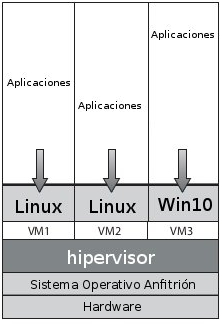
\includegraphics[width = 0.42\textwidth]{../architecture/v1/diagrams/virtualmachine}
\end{figure}

\newpage
La segunda técnica es conocida como virtualización del sistema operativo. En esta técnica lo que se virtualiza es el sistema operativo completo el cual corre directamente sobre la maquina física. A este tipo de máquinas virtuales se les denomina contenedores, los cuales acceden por igual a todos los recursos del sistema (Figura \ref{fig:contenedores}). Esta técnica tiene una ventaja que es a su vez una desventaja: todas las máquinas virtuales usan el mismo Kernel que el sistema operativo, lo que reduce los errores y multiplica el rendimiento, pero a su vez solo puede haber un mismo tipo de sistema operativo en los contenedores, no se puede combinar Windows, Linux, Etc. Este sistema también es un acercamiento a lo que seria una virtualización nativa \footnote{Tipo de virtualización en que intervienen las características del hardware. Los fabricantes preparan, sobre todo, los procesadores para que maquinas virtuales puedan trabajar con ellos más directamente.}.\\

\begin{figure}[h]
    \centering
	\caption{Contenedores}
	\label{fig:contenedores}
	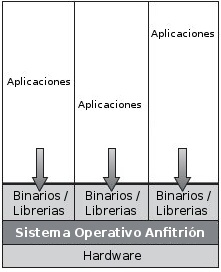
\includegraphics[width = 0.42\textwidth]{../architecture/v1/diagrams/contenedores}
\end{figure}

\newpage
De hecho, sin importar la técnica de virtualización que se use, la instalación de una maquina virtual (o de un contenedor) requiere normalmente de la generación e instalación de una imagen y a su vez de la instalación y configuración de paquetes de software. Estas tareas generalmente son realizadas por los técnicos de los proveedores de la nube. Cuando un usuario de la nube solicita un nuevo servicio o mas capacidad de computo, el administrador selecciona la imagen apropiada para clonar e instalar en los nodos de la nube. Si no existe una imagen apropiada para los requerimientos del cliente, se crea y configura una nueva que cumpla con la solicitud. Esta creación de una nueva imagen puede ser realizada modificando la imagen mas cercana de las ya existentes. En el momento de la creación optima de la imagen un administrador puede tener dificultades y preguntas como: ¿cuál es la mejor configuración?, ¿cuáles paquetes y sus dependencias deberían ser instaladas? y ¿cómo encontrar una imagen que mejor llene las expectativas?. Esto hace que la automatización y simplificación de este proceso sea una prioridad para los proveedores, ya que la depedencia entre entre paquetes de software y la dificultad de mantenimiento agrega tiempo a la creación de las máquinas virtuales. En otras palabras, uno de los principales objetivos de los proveedores de la nube es brindar mas flexibilidad y agilidad a la hora de satisfacer los requerimientos de los usuarios finales.\\
\\
\section{Soluciones de aprovisionamiento}
En el mercado existen muchas soluciones que permiten la interacción con diferentes ambientes de virtualización. Estas soluciones usan diferentes enfoques para realizar despliegues de software en las máquinas virtuales de manera rápida, controlada y automática. Sin embargo la mayoría de las soluciones no tienen la capacidad de manejar de manera simultanea las dos técnicas de virtualización antes mencionadas, algunas se centran solo en manejar máquinas virtuales y otras pocas solo hacen aprovisionamiento sobre contenedores.\\
\\
Así mismo, hay soluciones de aprovisionamiento que han incorporado su propio lenguaje buscando mayor flexibilidad y fácil configuración de las tareas. Sin embargo, esto implica incorporar una curva de aprendizaje bastante alta, lo que se traduce en un gran esfuerzo inicial para contar con toda la infraestructura automatizada. En ese mismo orden de ideas, existen a su vez, soluciones cuya curva de aprendizaje es mucho menor lo que las hace mas atractivas para muchos ingenieros de Tecnologías de la Información (TI).\\
\\
Adicionalmente, así como se encuentran soluciones o herramientas de aprovisionamiento de desarrollo propietario que cobran por sus funcionalidades mas importantes o por el numero de máquinas que pueden aprovisionar, existen herramientas de código abierto o de uso libre que permiten trabajar con un número considerable de máquinas virtuales. Al revisar alrededor de 40 diferentes herramientas de aprovisionamiento se logro identificar dos características que no se encuentran en las soluciones actuales. La primera trata de la ausencia de una interfaz o API \footnote{ API: Application Programming Interface, conjunto de subrutinas, funciones y procedimientos que ofrece un software para ser utilizado por otro software como una capa de abstracción.} web para realizar aprovisionamiento remoto y la segunda se refiere a que las herramientas se limitan a aprovisionar las máquinas virtuales sin ofrecer mecanismos de administración y monitoreo de la red aprovisionada o de los anfitriones que albergan los recursos virtuales.\\
\\
A continuación se describirán algunas de las herramientas mas conocidas actualmente son descritas a continuación:

\begin{description}
\item [Fabric]
 es una herramienta de automatización que usa SSH \footnote{SSH (Secure SHell, en español: intérprete de órdenes seguro) es el nombre de un protocolo y del programa que lo implementa, y sirve para acceder a máquinas remotas a través de una red} para hacer despliegues de aplicaciones y administración de tareas. Fabric es una librería gratuita hecha en python y su forma de interactuar es por medio de linea de comandos. Por otra parte permite cargar y descargar archivos que pueden ser ejecutados por su conjunto de funciones \cite{fabfile16}.

\item [Chef]
es una de las herramientas más conocidas de automatización de infraestructura de nube, esta escrita en Ruby y Erlang. Utiliza un lenguaje de dominio especifico, expresado también en Ruby para la escritura y configuracion de los recursos que deben ser creados, a esto se le denomina "recetas". Estas recetas contienen los recursos que deben ser creados. Chef se puede integrar con plataformas basadas en la nube, como Rackspace, Internap, Amazon EC2, Cloud Platform Google, OpenStack, SoftLayer y Microsoft Azure. Adicionalmente puede aprovisionar sobre contenedores si se instala la librería indicada. \\
\\
Chef contiene soluciones para sistemas de pequeña y gran escala \cite{Chef15}.Es uno de los cuatro principales sistemas de gestión de configuración en Linux, junto con Cfengine, Bcfg2 y Puppet. La version gratuita puede ser utilizada, pero no cuenta con todo el conjunto de caracteristicas, administracion y soporte brindados por la herramienta. Estos se pueden obtener pagando una licencia de uso.


\item [Puppet]
es una herramienta diseñada para administrar la configuración de sistemas similares a Unix y a Microsoft Windows de forma declarativa. El usuario describe los recursos del sistema y sus estados utilizando el lenguaje declarativo que proporciona Puppet. Esta información es almacenada en archivos denominados manifiestos Puppet. Puppet descubre la información del sistema a través de una utilidad llamada Facter, y compila los manifiestos en un catalogo especifico del sistema que contiene los recursos y las dependencias de dichos recursos, estos catálogos son ejecutados en los sistemas de destino \cite{Pupet15}. Puppet es de uso gratuito para redes muy pequeñas de hasta solo 10 nodos.

\item [Juju]
 es una herramienta de configuración y administración de servicios en nubes publicas. Permite crear ambientes completos con unos pocos comandos, cuenta con cientos de servicios pre-configurados y disponibles en la tienda de juju. Se puede usar a través de una interfaz gráfica o de linea de comandos. Juju permite re-crear un ambiente de producción en portátiles usando contenedores enfocado a pruebas. El uso de juju es gratuito pero se debe pagar por el uso de la nube publica \cite{juju16}.

\item [CFEngine]
es un sistema basado en el lenguaje escrito por Mark Burgess, diseñado específicamente para probar y configurar software. CFEngine es como un lenguaje de muy alto nivel. Su objetivo es crear un único archivo o conjunto de archivos que describen la configuración de cada máquina de la red. CFEngine se ejecuta en cada host, y analiza cada archivo (o archivos), que especifica una política para la configuración del sistema. La configuración de la máquina es verificada contra el modelo y, si es necesario, cualquier desviación de la configuración es corregida. \cite{cfengine15}\\
\\
CFEngine cuenta con una versión gratuita y la versión empresarial que cuenta con interfaz gráfica, soporte y reportes.

\item [Ansible]
es una herramienta de código libre desarrollada en python y comercialmente ofrecida por AnsibleWorks los cuales la definen como un motor de orquestación muy simple que automatiza las tareas de despliegue. Ansible no usa agentes, solo necesita tener instalado Python en las máquinas hosts y las tareas las realiza por medio de ssh. Ansible puede trabajar mediante un solo archivo de configuración que contendría todo o por medio de varios archivos organizados en una estructura de directorios \cite{ans16}. 

\item [Bcfg2]
esta escrito en Python y permite gestionar la configuración de un gran numero de ordenadores mediante un modelo de configuración central. Bcfg2 funciona con un modelo simple de configuración del sistema, modelando elementos intuitivos como paquetes, servicios y archivos de configuración (así como las dependencias entre ellos). Este modelo de configuración del sistema se utiliza para la verificación  y validación de las máquinas, permitiendo una auditoria robusta de los sistemas desplegados. La especificación de la configuración de Bcfg2 está escrita utilizando un modelo XML declarativo. Toda la especificacion puede ser validada utilizando los validadores de esquema XML ampliamente disponibles. Bcfg2 no tiene soporte para contenedores. Es gratuito y cuenta con una lista limitada de plataformas en las cuales trabaja bien.\cite{bdfg215}

\item [Cobbler]
 es una plataforma que busca el rápido despliegue de servidores y en general computadores en una infra-estructura de red por medio de linea de comandos, se basa en el modelo de scripts y cuenta con una completa base de simples comandos, que permite hacer despliegues de manera rápida y con poca intervención humana. Cobbler es capaz de instalar máquinas físicas y máquinas virtuales. Cobbler, es una pequeña y ligera aplicacion, que es extremadamente facil de usar para pequeños o muy grandes despliegues. Es de uso gratuito y no cuenta con soporte para contenedores. \cite{Cobbler15}

\item [SmartFrog]
 es un framework para servicios de configuración, descripción, despliegue y administración del ciclo de vida de máquinas virtuales. Consiste de un lenguaje declarativo, un motor que corre en los nodos remotos y ejecuta plantillas escritas en el lenguaje de SmartFrog y un modelo de componentes. El lenguaje soporta encapsulación (que es similar a las clases de python), herencia y composición que permite personalizar y combinar configuraciones. SmartFrog, permite enlaces estáticos y dinámicos entre componentes, que ayudan a soportar diferentes formas de conexión en tiempo de despliegue.\\
\\
El modelo de componentes, administra el ciclo de vida a través de cinco estados: instalado, iniciado, terminado y fallido. Esto permite al motor del SmartFrog detectar fallas y reiniciar automáticamente re-despliegues de los componentes \cite{Smart09}.\\
\\
SmartFrog es desarrollado y mantenido por un equipo de investigación en los laboratorios de Hewlett-Packard en Bristol, Inglaterra, así como por el laboratorio Europeo de Hewlett-Packard y por contribuciones de otros usuarios de SmartFrog y desarrolladores externos a HP. Se utiliza en la investigación de HP, específicamente en la automatización de la infraestructura y automatización de servicios, ademas de ser solo utilizado en determinados productos de HP.

\item [Amazon EC2]
es un API propietario de Amazon que maneja un enfoque manual, el cual permite desplegar imágenes de máquinas virtuales conocidas como AMI (Amazon Machine Images) \cite{Amazon16}, que son las imágenes que se utilizan en Amazon para arrancar instancias virtuales. El concepto de las AMIs \footnote{La AMI de Amazon es una imagen mantenida y compatible que ofrece Amazon Web Services para su uso en Amazon Elastic Compute Cloud (Amazon EC2).} es similar a las máquinas virtuales de otros sistemas. Básicamente estan compuestas de una serie de ficheros de datos que conforman la imagen y luego un xml que especifica ciertos valores necesarios para que sea una imagen valida para Amazon. 

\item [Docker composer]
permite describir un conjunto de contenedores que se relacionan entre ellos. Docker composer define una aplicación multicontenedor en un archivo con las mismas propiedades que se indicarían en un archivo individual de docker. Docker composer usa archivos en formato yaml para describir las características de los servicios en cada contenedor \cite{doccom16}. Es completamente gratuito. 

\item [Vagrant]
 es una herramienta de linea de comando que permite la creación y configuración de entornos de desarrollo virtualizados. Originalmente se desarrolló para VirtualBox y sistemas de configuración tales como Chef, Salt y Puppet. Sin embargo desde la versión 1.1 Vagrant es capaz de trabajar con múltiples proveedores, como VMware, Amazon EC2, LXC y DigitalOcean \cite{Vag15}.\\
\\
Vagrant ofrece múltiples opciones para realizar aprovisionamientos, desde scritps en shell hasta complejos sistemas de configuración.

\item [SaltStack]
 es un sistema de manejo de configuración cuyo objetivo es garantizar que un servicio este corriendo o que una aplicación haya sido instalada o desplegada. Salt está construido en Python y al igual que Chef, CFEngine y Puppet utiliza un esquema de cliente (salt minions) - servidor (salt master), cuyo método de conexión con los minions se realiza a través de un broker messages \footnote{es un programa intermediario que traduce los mensajes de un sistema desde un lenguaje a otro, a través de un medio de telecomunicaciones.} llamado ZeroMQ (0MQ), que no solo garantiza una conexión segura sino que la hace confiable y rápida. Salt tiene una versión gratuita llamada Salt Open sin embargo para obtener todos los beneficios se debe pagar la versión empresarial. Salt cuenta con soporte para contenedores. \cite{Salt15}

\end{description}
